\documentclass[a4paper,12pt]{article}
\usepackage[T1]{fontenc}
\usepackage[utf8]{inputenc}
\usepackage{lmodern}
\usepackage[french]{babel}
\usepackage{url,csquotes}
\usepackage[hidelinks,hyperfootnotes=false]{hyperref}
\usepackage[titlepage]{polytechnique}
%\usepackage[titlepage,fancysections,pagenumber]{polytechnique}
\usepackage{float}
\usepackage{graphicx}
\usepackage{subfig}
\usepackage{tocloft}

\usepackage{tcolorbox}

\usepackage{titlesec}

% Define the font size for subsection headings
\titleformat{\subsubsection}
{\large\bfseries}{\thesubsubsection}{1em}{}

%\setcounter{tocdepth}{}
%\usepackage[charter]{mathdesign}

%\setcounter{secnumdepth}{0}


\title{Proposition détaillée}
\subtitle{Modélisation de la congestion portuaire à l’aide de GNN temporel}
\author{Isai Gordeev\\
Promotion X2022\\INF11}

\usepackage{hyperref}



\begin{document}

\maketitle



\tableofcontents

\newpage

\section{Les enjeux et la motivation du travail proposé}

CMA CGM est une grande entreprise de logistique, la deuxième plus grande entreprise de transport de navires et de conteneurs au monde. L’une des tâches naturelles du travail de l’entreprise consiste à prédire l’état de tous les ports disponibles dans le système d’approvisionnement des navires. À l'heure actuelle, l'approvisionnement des navires comporte deux tâches fondamentales : prévoir le nombre de navires en attente au port et le temps d'attente du navire. Ces problèmes sont résolus à l'aide d'algorithmes ML classiques, tels que des modèles de régression ponctuelle pour chaque port. Nous proposons d'utiliser un GNN temporel pour modéliser tous les ports disponibles en fonction de ces raisons. GNN est une branche de DL qui est encore en développement et le potentiel de ces réseaux n'a pas été exploité. Compte tenu des progrès récents dans les mécanismes d’attention et les CNN, les GNN restent très intéressants car ces mécanismes apparaissent naturellement dans les GNN.

\section{La revue et une analyse de l’état de l’art ainsi que des approches concurrentes et alternatives}





\section{Les objectifs intermédiaires et leur échéancier}

Comprendre les subtilités de la théorie.
Les techniques courantes de l'apprentissage. 
Découvrir plus de state of art modeles. 
Le premier tâche c'est de trouver le balance sur embedding, architecture du GNN. 


\section{L’organisation du travail et la répartition du travail}

Nous somme 4 dans l'équipe. 


\section{L'identification des moyens auxquels le projet fera appel}

Nous utiliserons des ordinateurs portables personnels pour écrire et implémenter le code car nous travaillerons sur le projet à distance. Nous utiliserons les services internes de CMA CGM pour stocker et compiler les projets, et nous utiliserons Google Colab pour les brouillions de modèles d'architecture. Possiblement pour la taille de notre architectures il nous faudra acheter une souscription pour avoir accès aux GPU plus puissants avec le stockage de poids des réseaux. Nous utiliserons également Microsoft Teams pour communiquer avec le tuteur.

Pour entraîner les réseaux de neurones, l'entreprise fournira les ressources informatiques nécessaires avec une architecture GPU, que nous utiliserons à distance sur le serveur pour tester nos architectures. Sur demande, nous utiliserons également des services open source pour le débogage des réseaux de neurones et des systèmes de contrôle de version pour les architectures.

	
\section{Conclusion}

Dans ce rapport, j'ai décrit 

%\begin{figure}[htbp]
%	\centering
%	\begin{minipage}{0.3\textwidth}
%		\centering
%		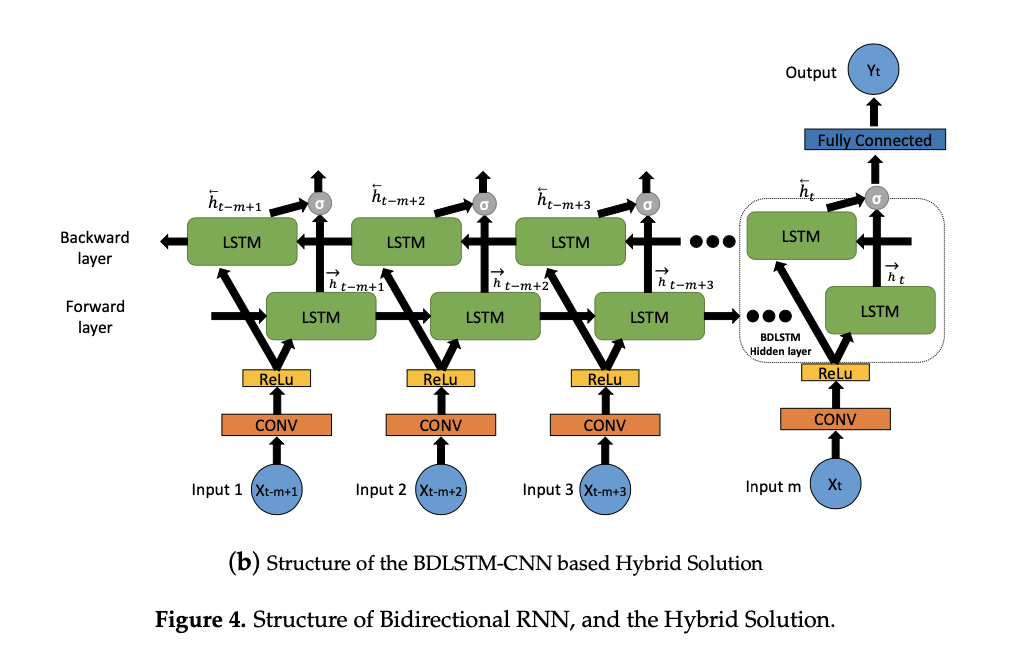
\includegraphics[width=\linewidth]{3}
%		\caption{Nos photos que Patrick a accrochées à son mur en souvenir de l'événement.}
%		\label{fig:image1}
%	\end{minipage}
%	\hfill
%	\begin{minipage}{0.3\textwidth}
%		\centering
%		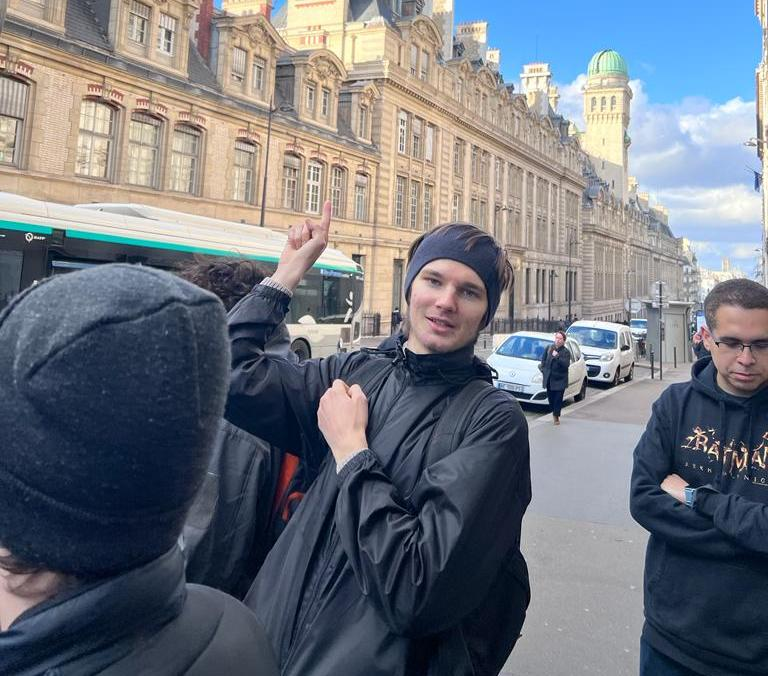
\includegraphics[width=\linewidth]{33}
%		\caption{Je montre le mur d'obus lors d'une randonnée dans le Quartier Latin}
%		\label{fig:image2}
%	\end{minipage}
%	\hfill
%	\begin{minipage}{0.3\textwidth}
%		\centering
%		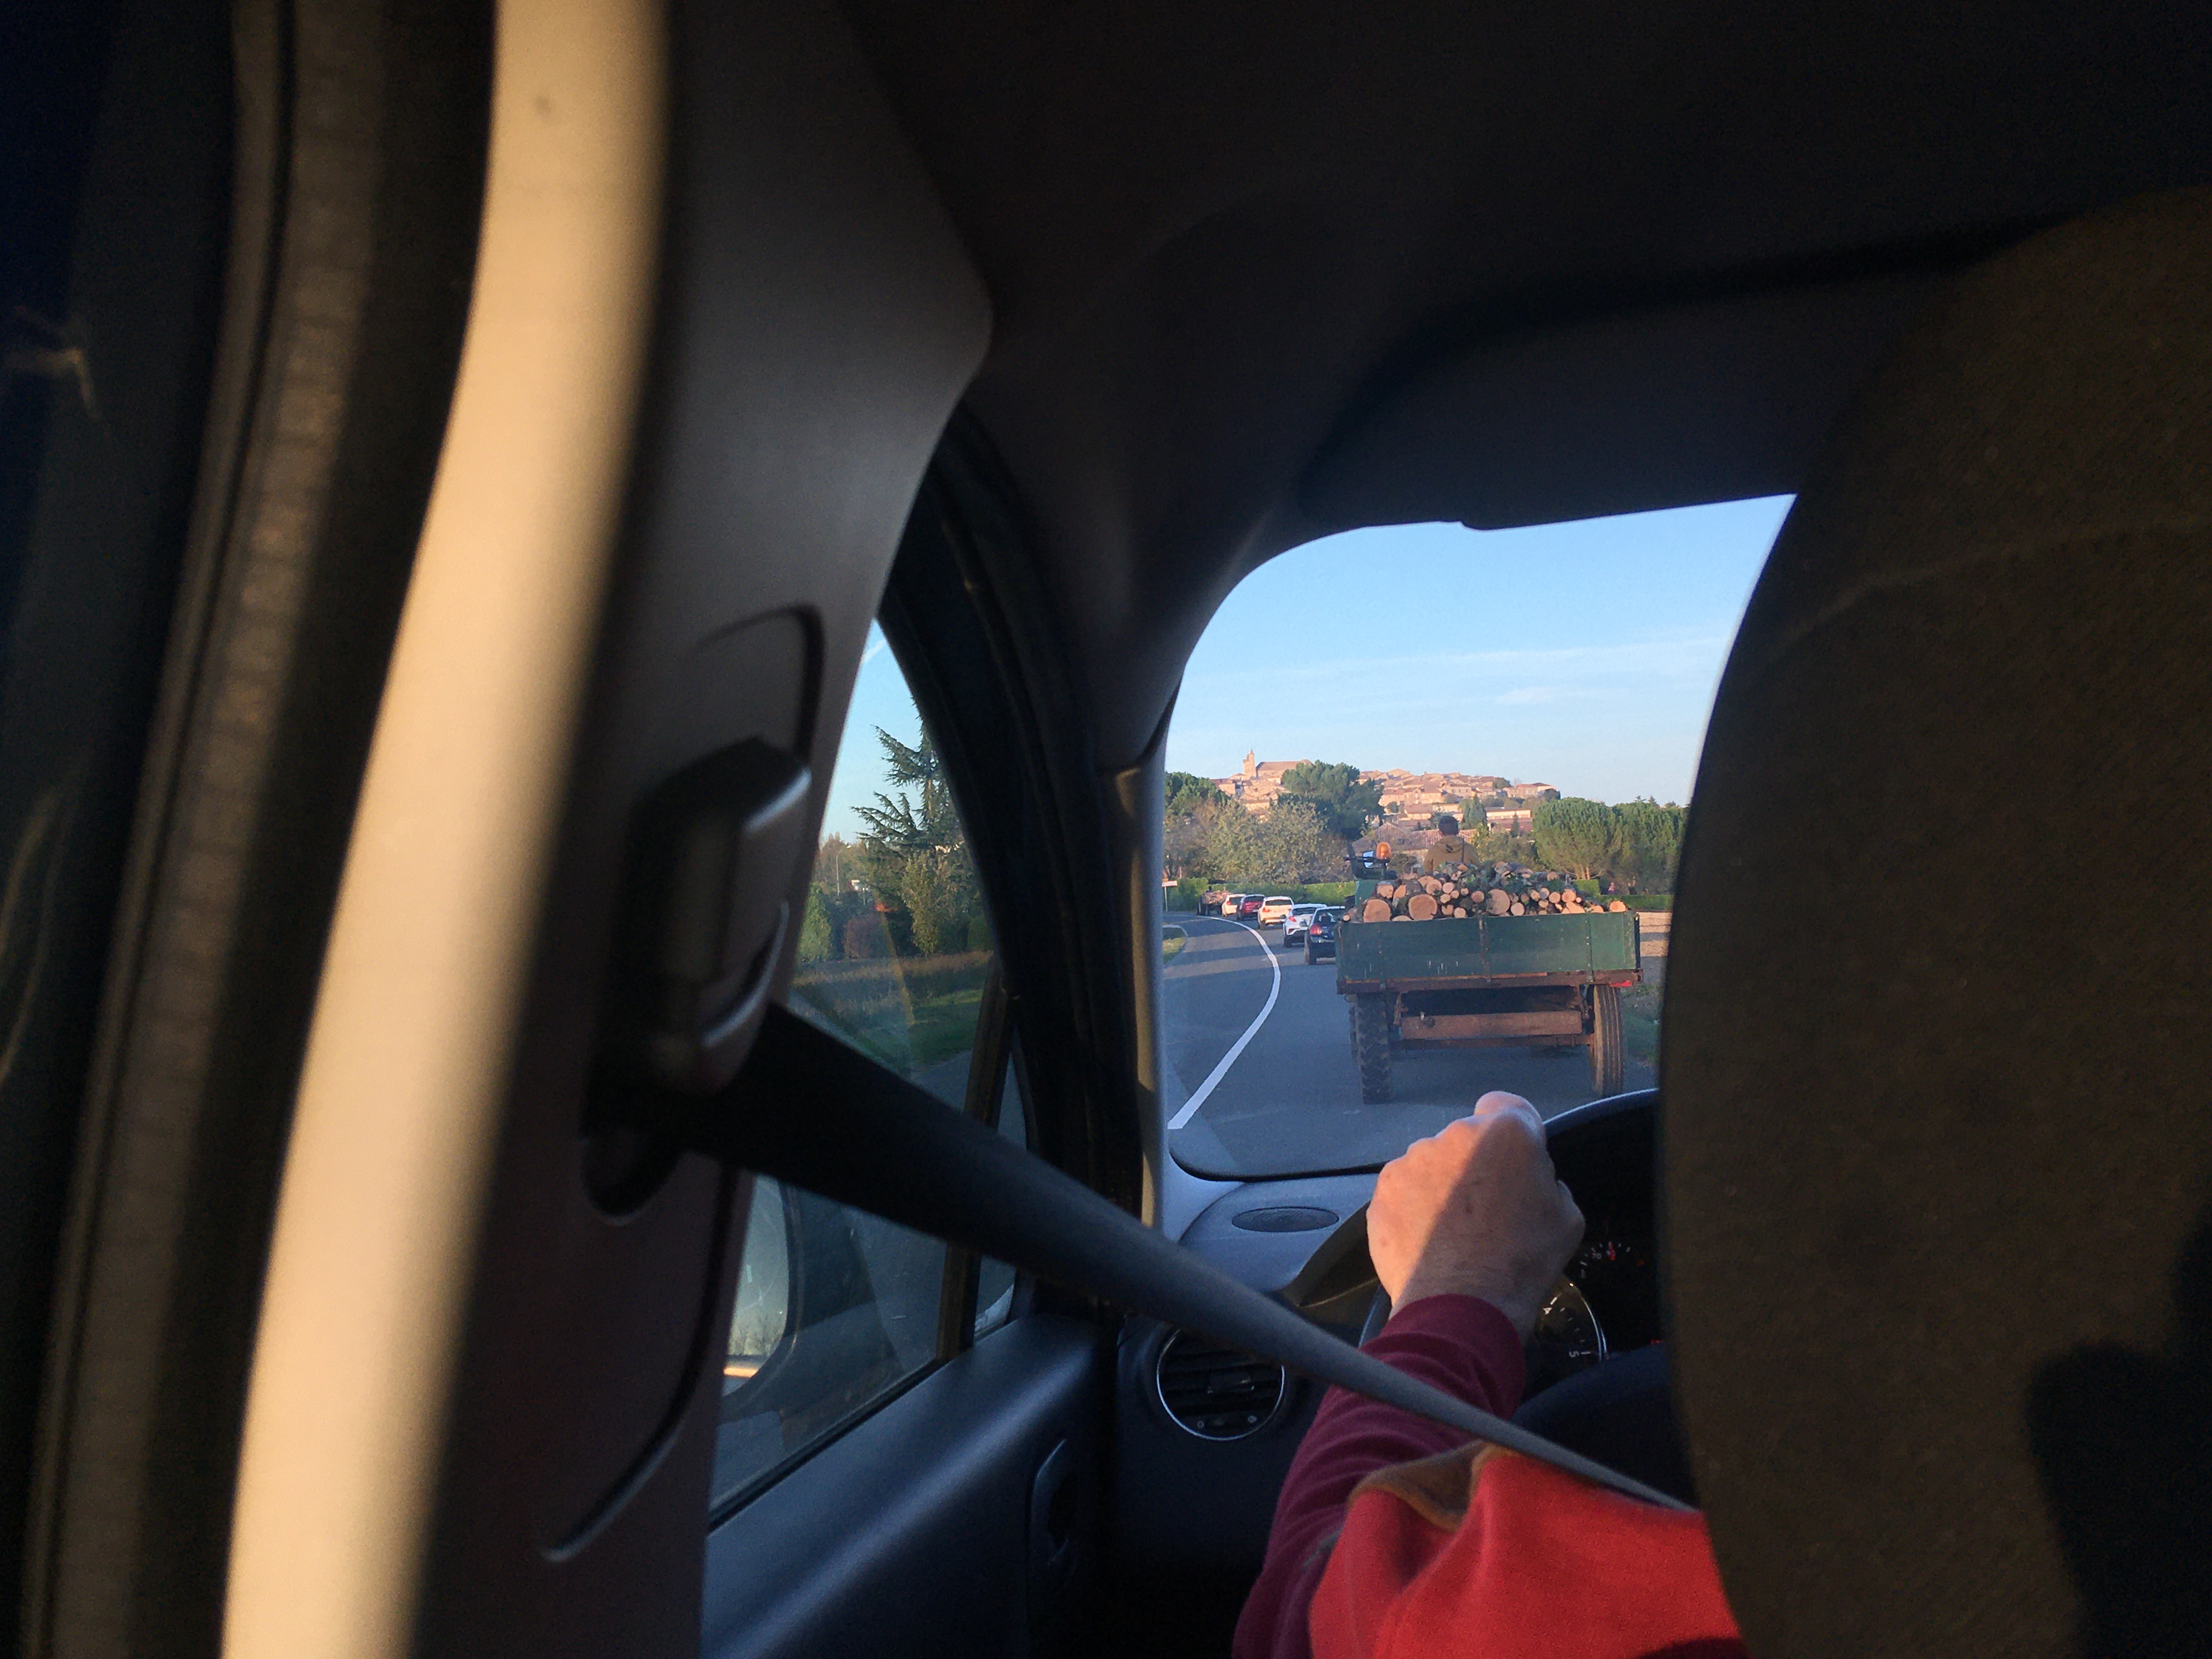
\includegraphics[width=\linewidth]{321}
%		\caption{Patrick nous emmène dans un village vieux de 1000 ans.}
%		\label{fig:image3}
%	\end{minipage}
%	\label{fig:myfigure}
%\end{figure}
%
%\begin{figure}[htbp]
%	\centering
%	\begin{minipage}{0.3\textwidth}
%		\centering
%		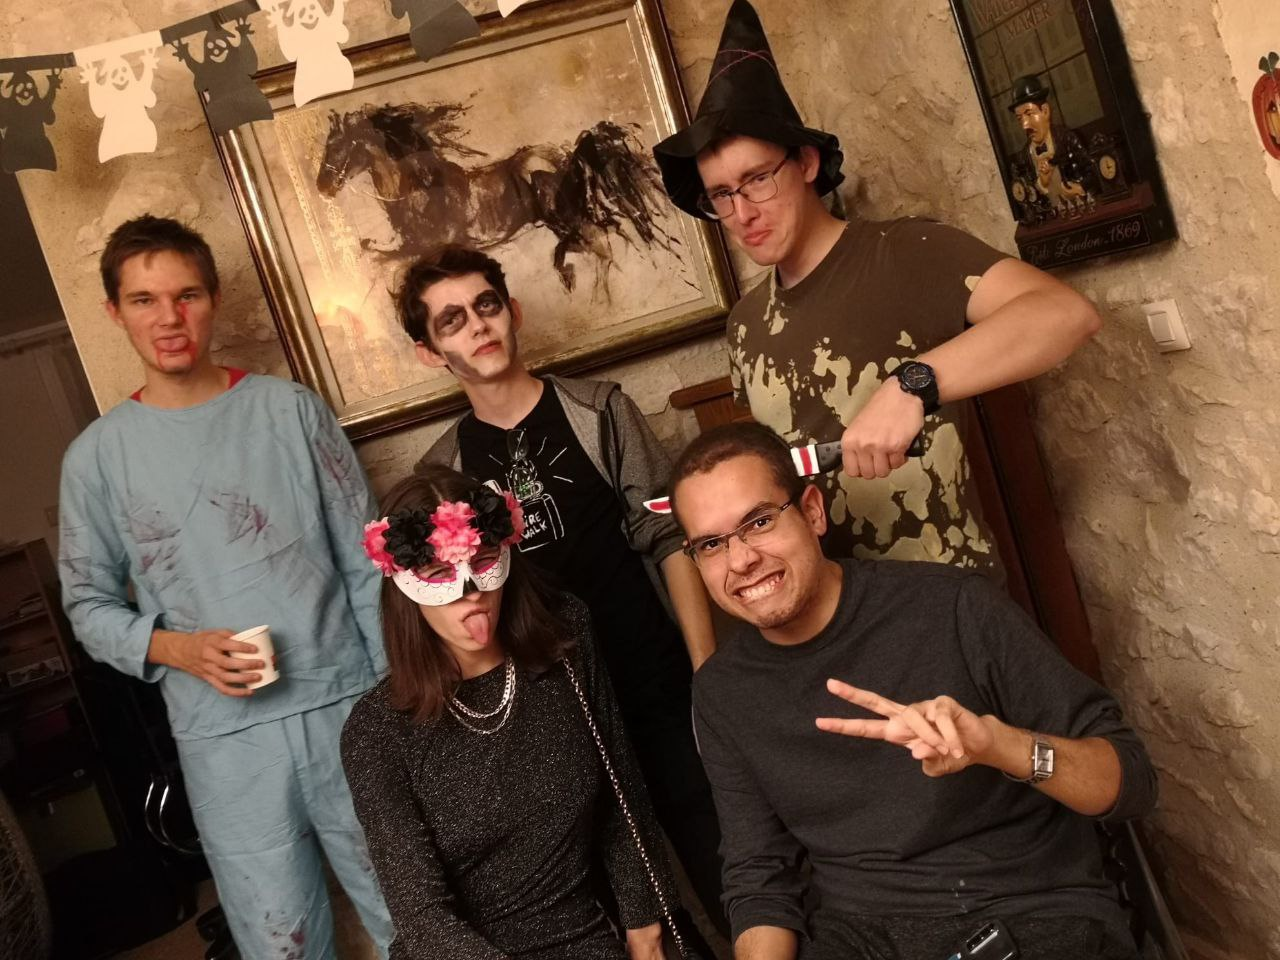
\includegraphics[width=\linewidth]{4}
%		\caption{À l'occasion de Halloween dans la famille d'accueil de mon ami}
%		\label{fig:image1}
%	\end{minipage}
%	\hfill
%	\begin{minipage}{0.3\textwidth}
%		\centering
%		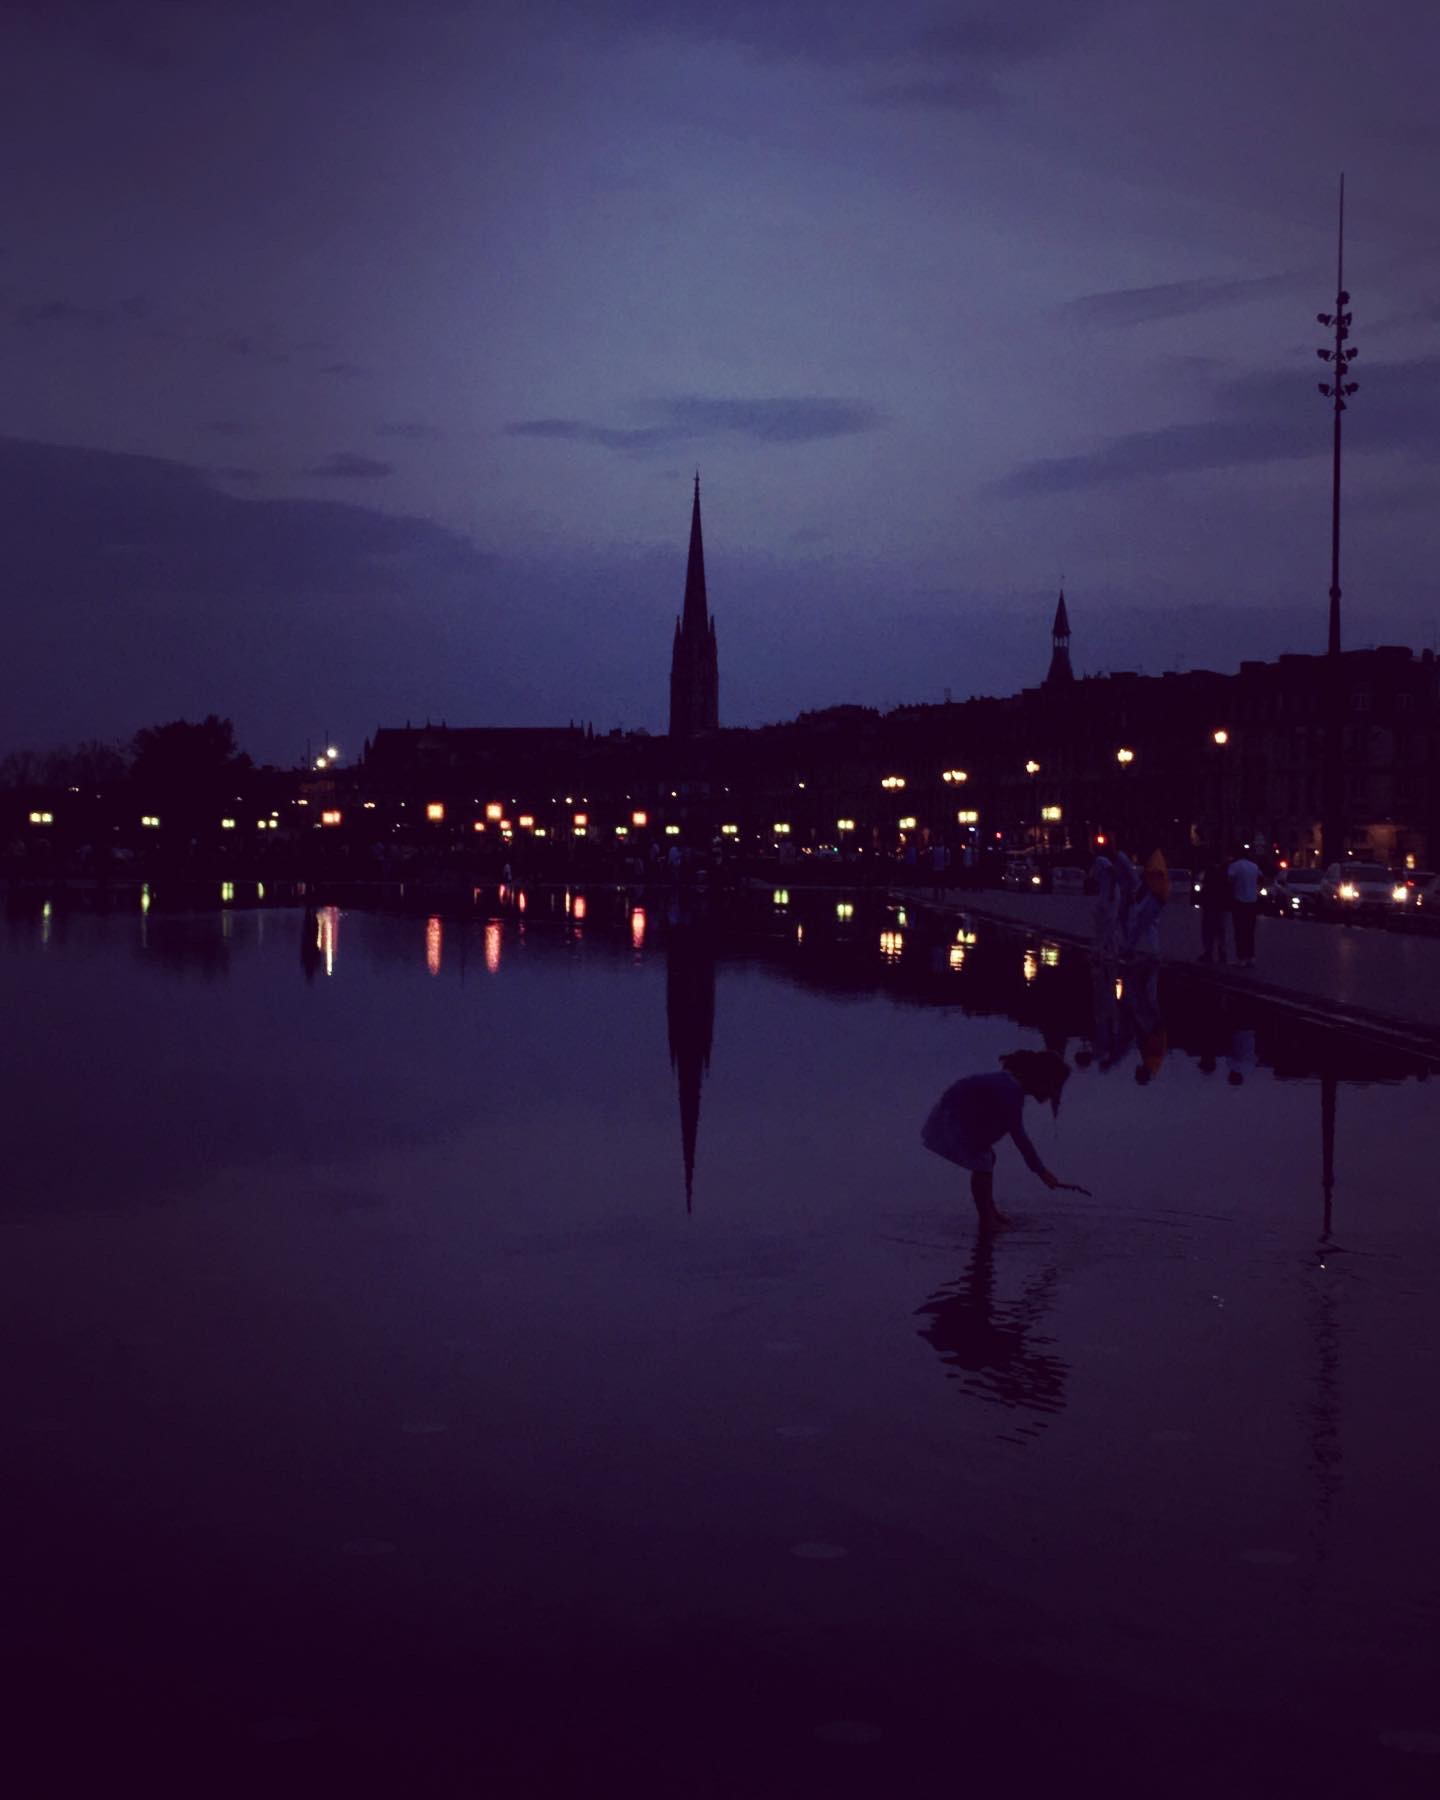
\includegraphics[width=\linewidth]{43}
%		\caption{La photo prise à Bordeaux lors d'un week-end à Villeneuve}
%		\label{fig:image2}
%	\end{minipage}
%	\hfill
%	\begin{minipage}{0.3\textwidth}
%		\centering
%		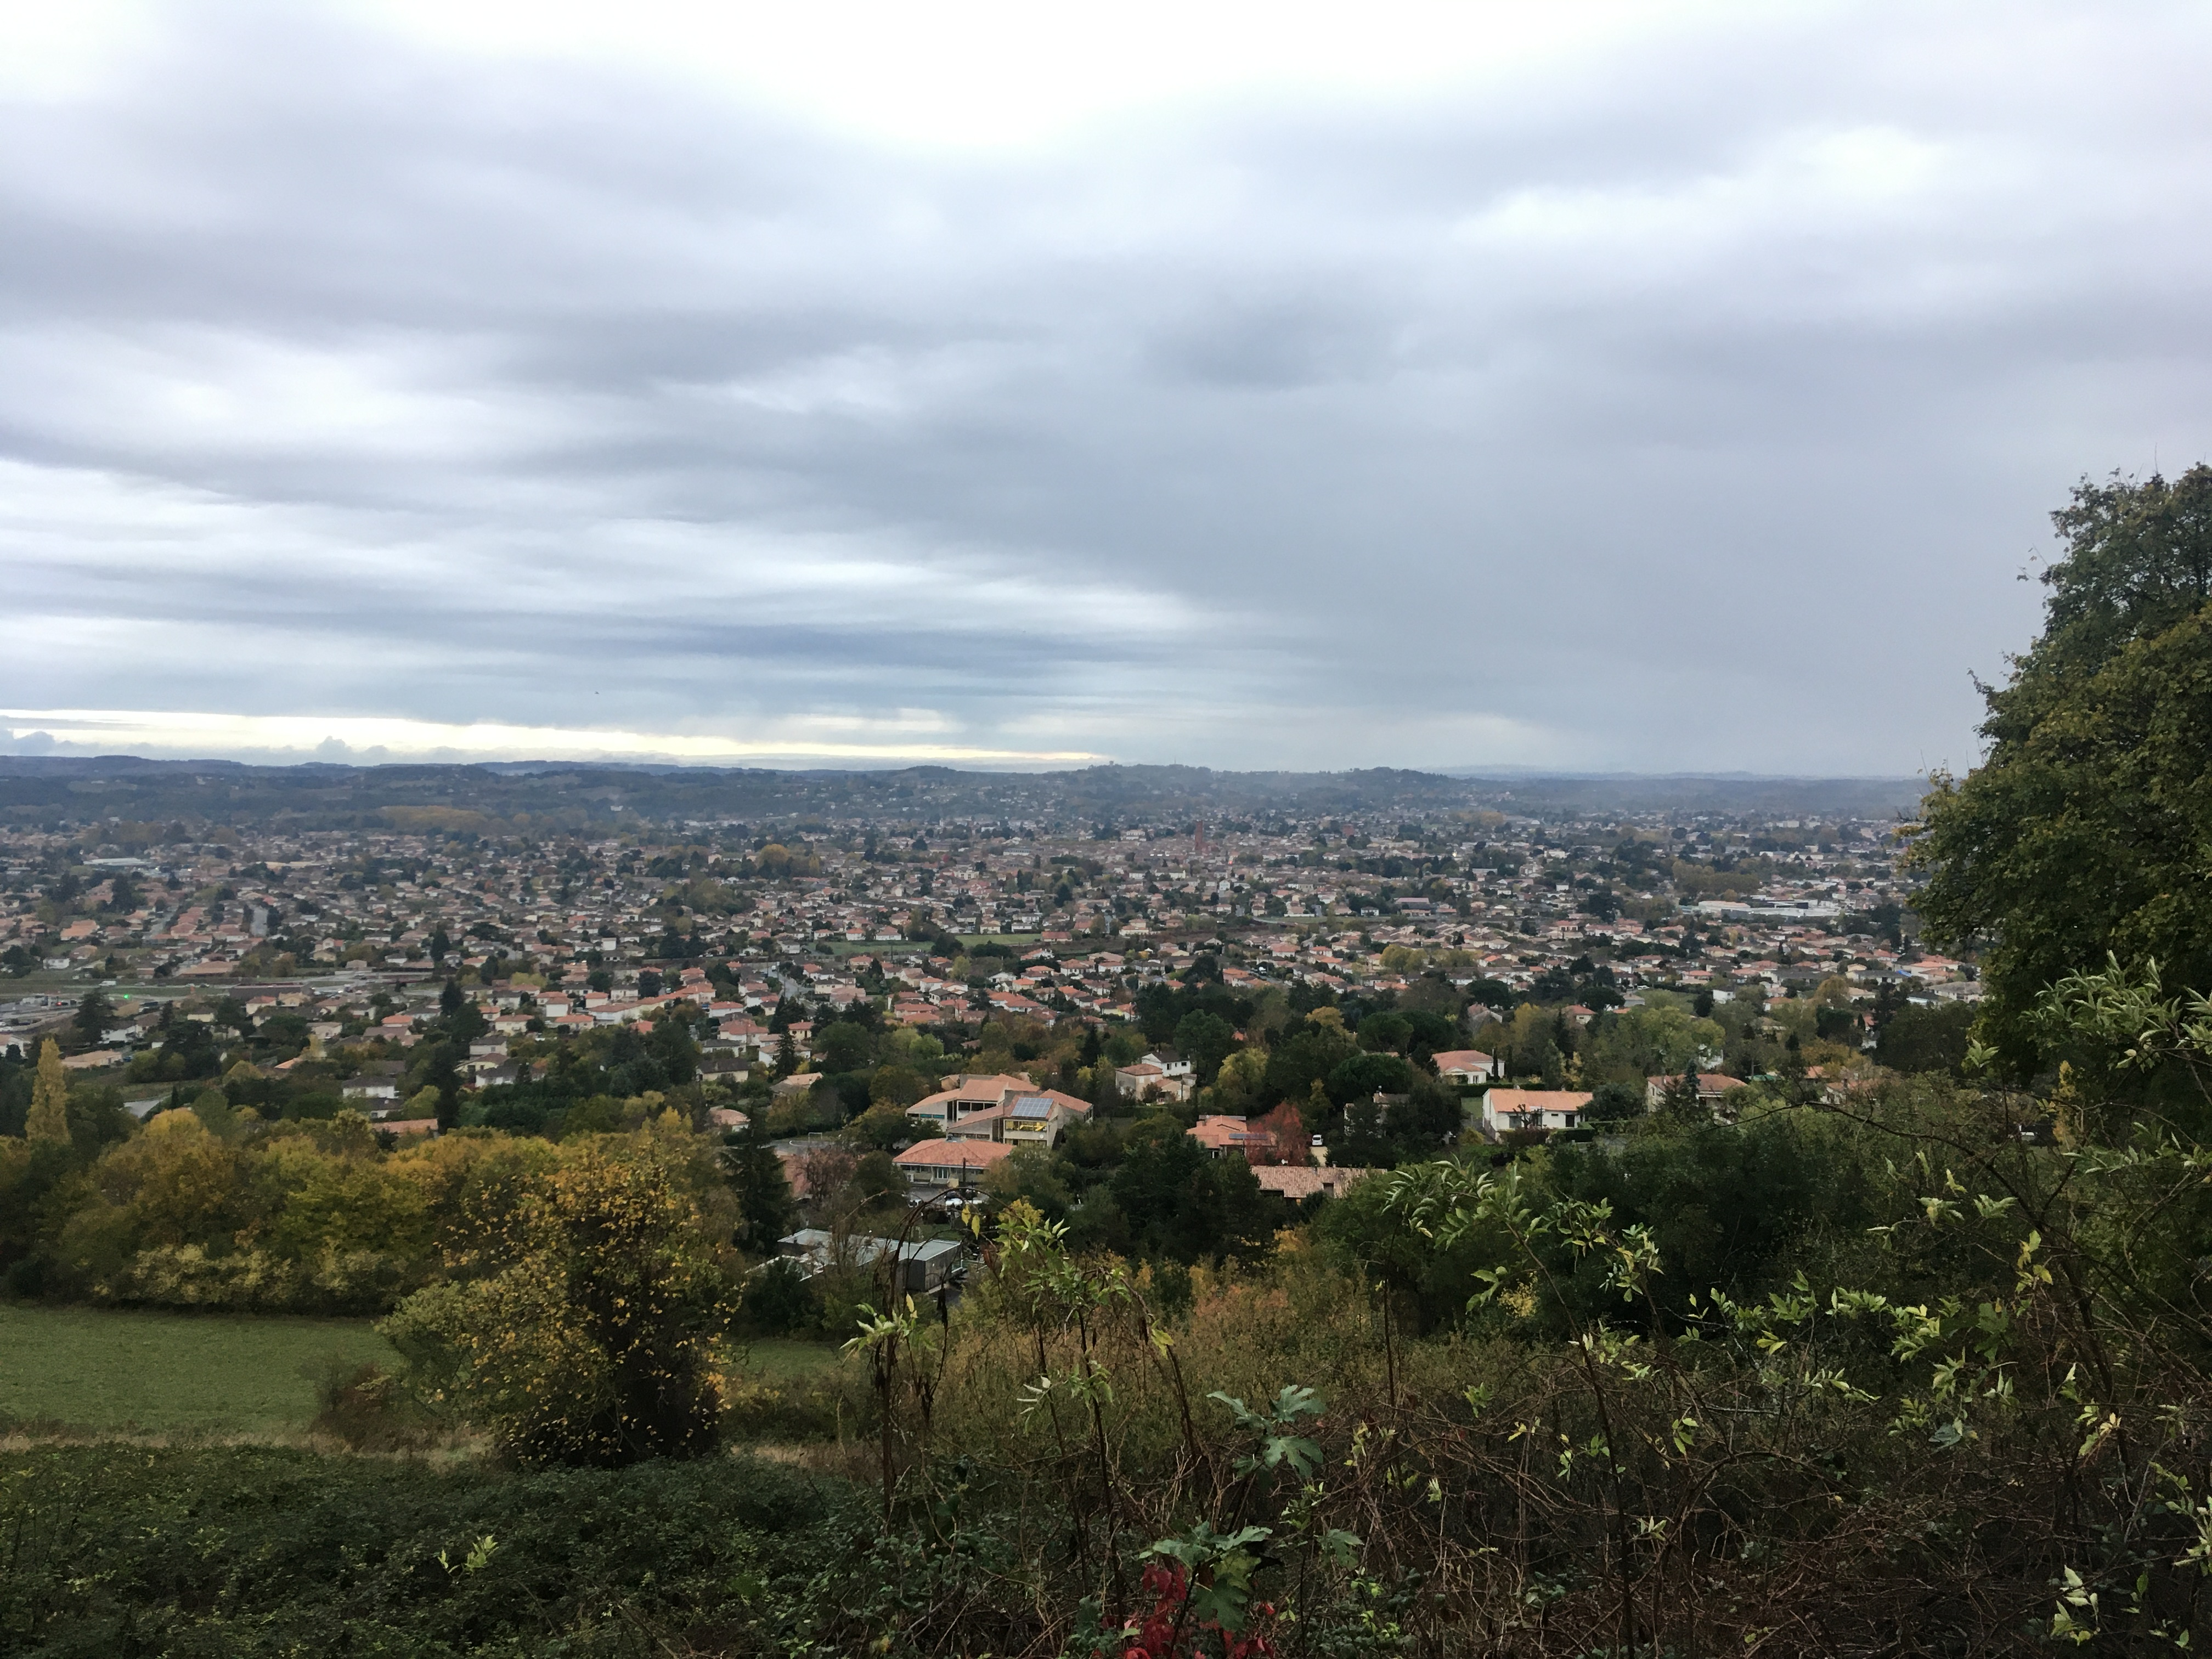
\includegraphics[width=\linewidth]{123}
%		\caption{Une photo de Villeneuve que j'ai prise lors de ma promenade}
%		\label{fig:image3}
%	\end{minipage}
%	\label{fig:myfigure}
%\end{figure}

\end{document}